%&pdflatex
\section{Scrittura su pendrive USB}
Per scrivere un file immagine ISO su un pendrive USB da Microsoft Windows, Apple OS X o Linux (per Linux è anche disponibile l'utility \texttt{dd} che è molto più flessibile) è possibile utilizzare \texttt{UNetbootin}:

\begin{graybox}
	https://unetbootin.github.io
\end{graybox}

Inseriamo un pendrive vuoto (tutti i dati presenti sopra saranno cancellati!) e apriamo UNetbootin. Notiamo che è anche possibile chiedere a UNetbootin di scaricare per noi la distribuzione che vogliamo scrivere sul pendrive. Dato che abbiamo già scaricato Debian, scegliamo \texttt{Immagine disco} e specifichiamo l'immagine di Debian --- come mostrato in Figura \vref{fig:unetbootin}.

\begin{figure}[ht]
	\centering
	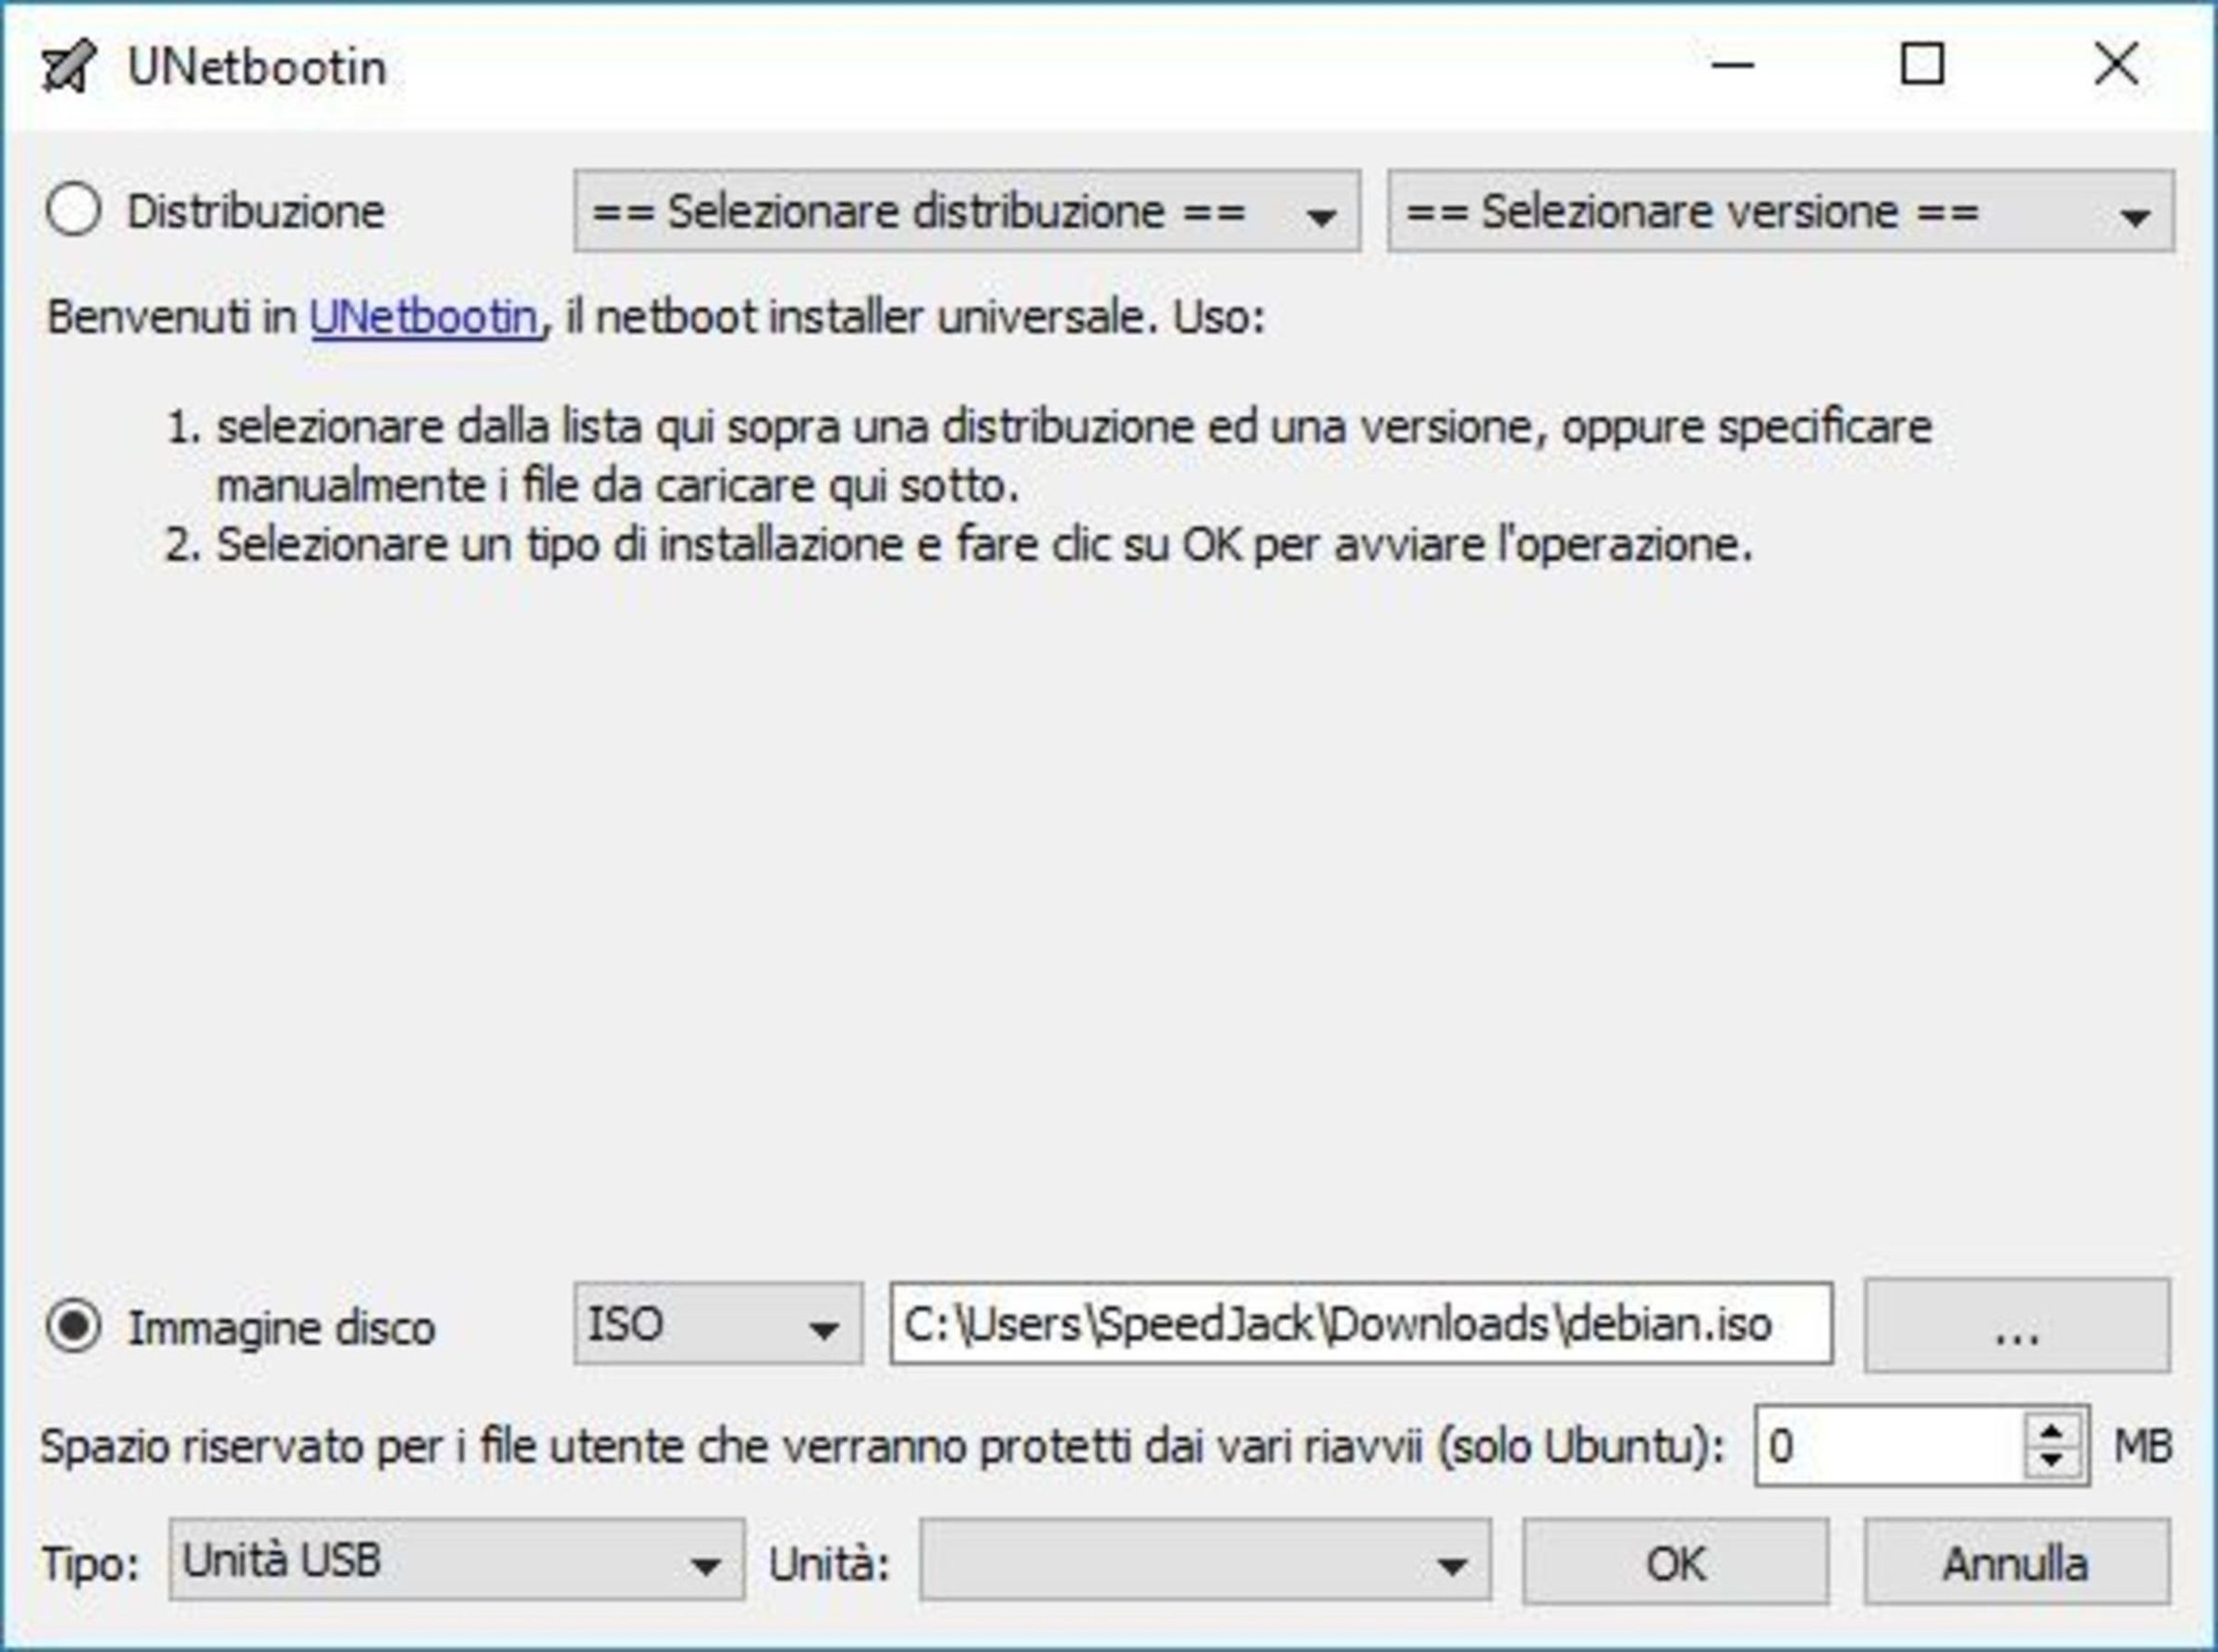
\includegraphics[resolution=600]{unetbootin}
	\caption{Scrittura di un pendrive USB con \texttt{UNetbootin}}
	\label{fig:unetbootin}
\end{figure}

Clicchiamo quindi su \texttt{OK}. Al termine, avremo un pendrive USB con Debian pronto per essere avviato!
